\documentclass[11pt,a4paper]{article}
\usepackage[margin=2cm]{geometry}
\usepackage{titlesec}
\usepackage{booktabs}
\usepackage{array}
\usepackage{enumitem}
\usepackage{xcolor}
\usepackage{mdframed}
\usepackage{hyperref}
\usepackage{parskip}
\usepackage{tabularx}
\usepackage{multicol}
\usepackage{tikz}
\usetikzlibrary{shapes.geometric, arrows.meta, positioning}

\definecolor{examblue}{RGB}{30,80,160}
\definecolor{keyred}{RGB}{180,30,30}
\definecolor{notegreen}{RGB}{20,120,60}
\definecolor{bglight}{RGB}{245,248,255}
\definecolor{slidegray}{RGB}{90,90,90}

\titleformat{\section}{\large\bfseries\color{examblue}}{}{0em}{}[\titlerule]
\titleformat{\subsection}{\normalsize\bfseries\color{keyred}}{}{0em}{}

\setlist[itemize]{noitemsep, topsep=2pt, leftmargin=*}
\setlist[enumerate]{noitemsep, topsep=2pt, leftmargin=*}

\newmdenv[backgroundcolor=bglight, linecolor=examblue, linewidth=1pt,
  innertopmargin=4pt, innerbottommargin=4pt, skipabove=6pt, skipbelow=4pt]{refbox}

\newmdenv[backgroundcolor={yellow!10}, linecolor=keyred, linewidth=1pt,
  innertopmargin=4pt, innerbottommargin=4pt, skipabove=4pt, skipbelow=4pt]{answerbox}

\newcommand{\qref}[1]{\textbf{\textcolor{examblue}{[#1]}}}
\newcommand{\mk}[1]{\textcolor{slidegray}{\small(#1 mk)}}
\newcommand{\key}[1]{\textbf{\textcolor{keyred}{#1}}}

\begin{document}

\begin{center}
{\LARGE\bfseries CSE 719 — Lecture 10: RPCs \& Concurrency Control}\\[4pt]
{\large Past-Paper Solutions (2020--2024)}\\[2pt]
{\normalsize Exam: Wed 1 Jul 2026 $\;\cdot\;$ Yield: 5/5 $\;\cdot\;$ $\approx$55+ marks covered}
\end{center}
\vspace{-4pt}\hrule\vspace{8pt}

%=============================================================
\section{Quick Reference}
%=============================================================

\begin{refbox}
\textbf{RPC:} Call from one function to another where caller and callee reside in \emph{different processes} (possibly different hosts). Procedure address = IP + port + procedure number. Counterpart: RMI in object-based settings. Proposed by Birrell \& Nelson (1984).

\textbf{Key RPC components:}
\begin{itemize}
  \item \key{Client stub} --- same function signature as callee; marshals arguments; allows same caller code for LPC and RPC
  \item \key{Communication module} --- forwards requests and replies to appropriate hosts
  \item \key{Dispatcher} --- selects which server stub to route the request to
  \item \key{Server stub} --- unmarshals arguments; calls callee; marshals return value
\end{itemize}

\textbf{Call semantics:}
\begin{center}
\begin{tabular}{lllll}
\toprule
Retransmit? & Filter dups? & Re-execute or Retransmit reply? & Semantics & Example \\
\midrule
Yes & No & Re-execute & At least once & Sun RPC \\
Yes & Yes & Retransmit reply & At most once & Java RMI \\
No & N/A & N/A & Maybe & CORBA \\
\bottomrule
\end{tabular}
\end{center}

\textbf{ACID:} Atomicity (all-or-nothing) · Consistency (server stays consistent) · Isolation (indivisible from other transactions) · Durability (committed effects survive crashes).

\textbf{Concurrency problems:} Lost Update (two txns overwrite each other) · Inconsistent Retrieval (txn reads partially updated data).

\textbf{Serial equivalence:} Interleaving is serially equivalent iff all pairs of conflicting operations from different transactions execute in the same order for every shared object. Conflict = same object, at least one write.

\textbf{Deadlock:} Circular wait. Detected via Wait-For-Graph (WFG). Prevented via 2PL or timestamp ordering.
\end{refbox}

%=============================================================
\section{RPC: Definition, Motivation, Design Issues}
%=============================================================
\qref{2021 Q8a \mk{2.75}, 2022 Q8a \mk{3}, 2020 Q3a \mk{1.5}}

\begin{answerbox}
\textbf{What is RPC?}

A \key{Remote Procedure Call (RPC)} is a mechanism that allows a function in one process (caller) to invoke a function residing in a \emph{different process} --- possibly on a different machine --- in the same way as a local procedure call, without the programmer explicitly coding the network communication.

\begin{itemize}
  \item Caller and callee are in different processes; the function call crosses a process boundary.
  \item Cannot use pointers across processes (address in P1 is meaningless in P2); instead uses \emph{global references}: IP address + port + procedure number.
  \item Object-based counterpart: \textbf{Remote Method Invocation (RMI)}.
  \item Code for client stub, dispatcher, server stub is \emph{generated automatically} from function signatures by middleware (CORBA, Sun RPC, Java RMI).
  \item Enables code reuse, transparency, and modularity in distributed systems.
\end{itemize}

\textbf{Primary motivation:} Allow processes to call functions in other processes with the same familiar call syntax as local calls, hiding all network complexity in the middleware layer. This enables distributed system construction through modular procedure invocation.

\textbf{Design Issues for RPC:}
\begin{enumerate}
  \item \key{Call semantics} --- Cannot guarantee exactly-once under failures. Must choose: at-most-once (filter duplicates, retransmit reply), at-least-once (retransmit + re-execute), or maybe (no retransmit).
  \item \key{Parameter passing / Marshalling} --- Caller and callee may use different data representations (big-endian vs little-endian). Middleware converts arguments to \emph{Common Data Representation (CDR)} before transmission (marshalling) and back on receipt (unmarshalling).
  \item \key{Binding} --- How does the client locate the server? Static binding (hardcoded) or dynamic binding (name server lookup at runtime).
  \item \key{Transport protocol} --- UDP (lightweight, needs RRA retransmit logic) vs TCP (reliable but heavier). Choice affects latency and failure handling.
  \item \key{Fault tolerance} --- Server may crash before or after executing the call; client cannot distinguish these cases. Need idempotent operations or unique request IDs.
  \item \key{Security} --- Authentication (is the server who it claims to be?) and authorization. RPCs cross trust boundaries.
  \item \key{Heterogeneity} --- Caller and callee may run on different OSes, languages, hardware. CDR and stub generation solve this.
  \item \key{Performance} --- RPC is much slower than LPC (network round trip, marshalling overhead). Must minimise unnecessary RPCs (e.g., AFS whole-file caching).
\end{enumerate}
\end{answerbox}

%=============================================================
\section{Schematic Diagram of RPC Mechanism}
%=============================================================
\qref{2020 Q3a \mk{3}}

\begin{answerbox}
\begin{center}
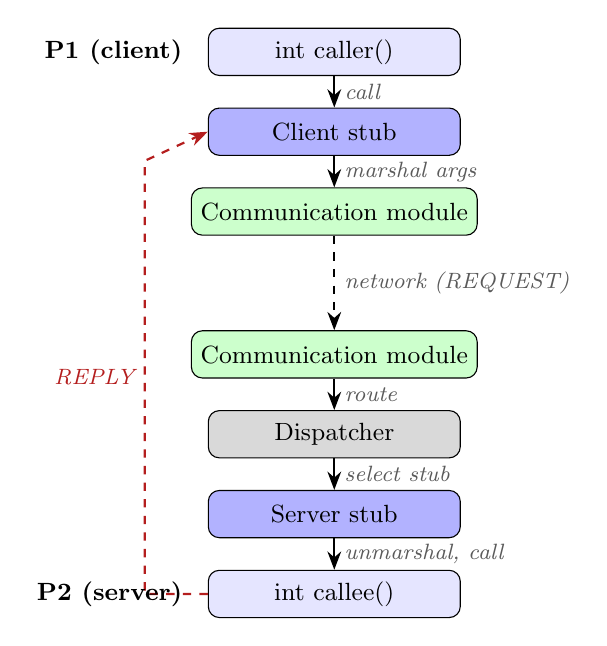
\begin{tikzpicture}[
  box/.style={draw, rounded corners, minimum width=3.2cm, minimum height=0.6cm, align=center, font=\small},
  arrow/.style={-Stealth, thick},
  label/.style={font=\footnotesize\itshape, color=slidegray}
]
% Client side (P1)
\node[box, fill=blue!10] (caller) {int caller()};
\node[box, fill=blue!30, below=0.4cm of caller] (cstub) {Client stub};
\node[box, fill=green!20, below=0.4cm of cstub] (ccomm) {Communication module};

% Server side (P2)
\node[box, fill=green!20, below=1.2cm of ccomm] (scomm) {Communication module};
\node[box, fill=gray!30, below=0.4cm of scomm] (disp) {Dispatcher};
\node[box, fill=blue!30, below=0.4cm of disp] (sstub) {Server stub};
\node[box, fill=blue!10, below=0.4cm of sstub] (callee) {int callee()};

% Arrows client side
\draw[arrow] (caller) -- node[right, label]{call} (cstub);
\draw[arrow] (cstub) -- node[right, label]{marshal args} (ccomm);

% Network arrow
\draw[arrow, dashed] (ccomm) -- node[right, label]{network (REQUEST)} (scomm);

% Arrows server side
\draw[arrow] (scomm) -- node[right, label]{route} (disp);
\draw[arrow] (disp) -- node[right, label]{select stub} (sstub);
\draw[arrow] (sstub) -- node[right, label]{unmarshal, call} (callee);

% Return path (left side)
\draw[arrow, color=keyred, dashed] (callee.west) -- ++(-0.8,0) -- node[left, label, color=keyred]{REPLY} ++(0,5.5) -- (cstub.west);

% Labels
\node[left=0.2cm of caller, font=\small\bfseries] {P1 (client)};
\node[left=0.2cm of callee, font=\small\bfseries] {P2 (server)};
\end{tikzpicture}
\end{center}

\begin{itemize}
  \item \textbf{Client stub}: has the same signature as \texttt{callee()}; allows \texttt{caller()} code to be identical whether making LPC or RPC.
  \item \textbf{Communication module}: forwards marshalled request to server host; receives reply, returns to stub.
  \item \textbf{Dispatcher}: on server, selects correct server stub based on procedure ID in the request message.
  \item \textbf{Server stub}: unpacks (unmarshals) arguments; invokes actual \texttt{callee()}; marshals return value into REPLY.
\end{itemize}
\end{answerbox}

%=============================================================
\section{Stub: What Is It, How Generated, and Its Purpose}
%=============================================================
\qref{2020 Q3b \mk{4.25}}

\begin{answerbox}
\textbf{What is a stub?}

A \key{stub} is a piece of middleware code that acts as a local proxy for a remote function. It has the \emph{same function signature} as the remote callee so that the caller can invoke it as if calling a local function --- hiding all network communication details.

There are two stubs:
\begin{itemize}
  \item \textbf{Client stub}: Lives in the caller's process. Marshals arguments into CDR format, sends the REQUEST message, waits for REPLY, unmarshals the result, and returns it to the caller.
  \item \textbf{Server stub}: Lives in the callee's process. Receives the REQUEST from the dispatcher, unmarshals arguments, calls the actual \texttt{callee()} function, marshals the return value, sends the REPLY.
\end{itemize}

\textbf{How are stubs generated?}

Stubs are \key{generated automatically} by a middleware compiler --- the programmer does \emph{not} write them by hand:
\begin{enumerate}
  \item Programmer defines the function interface in an \textbf{Interface Definition Language (IDL)} (e.g., Sun XDR for Sun RPC, CORBA IDL for CORBA).
  \item The IDL file is fed into a \textbf{stub compiler} (e.g., \texttt{rpcgen} for Sun RPC).
  \item The compiler outputs: client stub code, server stub code, and marshalling/unmarshalling routines for all parameter types.
  \item Programmer only writes: the \texttt{caller()} business logic and the \texttt{callee()} implementation.
\end{enumerate}

\textbf{Functionality and purpose of stubs:}
\begin{itemize}
  \item \textbf{Transparency}: The caller does not know whether it is invoking a local or remote function.
  \item \textbf{Marshalling}: Converts arguments from platform-dependent format to CDR; handles endianness, data type sizes, pointer elimination.
  \item \textbf{Call semantics enforcement}: Implements retransmit logic, duplicate detection, and reply caching to achieve at-most-once or at-least-once semantics.
  \item \textbf{Decoupling}: The programmer focuses on business logic; the stub handles all distributed systems complexity.
\end{itemize}
\end{answerbox}

%=============================================================
\section{RRA Protocol and Concurrent Extension}
%=============================================================
\qref{2020 Q5a (RRA steps + figure), 2020 Q5d \mk{2.75} (concurrent access to multiple servers)}

\begin{answerbox}
\textbf{Communication Protocol in RPC: the RRA Protocol}

The \key{Request-Reply-Acknowledge (RRA)} protocol is used by RPC over UDP to achieve reliable, at-most-once communication without TCP's overhead.

\textbf{Steps of RRA:}
\begin{enumerate}
  \item \textbf{Client sends REQUEST}: message contains $\langle$\textit{request\_id, procedure\_id, arguments}$\rangle$. The \textit{request\_id} uniquely identifies this invocation.
  \item \textbf{Server executes} the procedure. Server stores the result (reply) indexed by \textit{request\_id}.
  \item \textbf{Server sends REPLY}: message contains $\langle$\textit{request\_id, result}$\rangle$.
  \item \textbf{Client receives REPLY}, extracts result, returns to caller.
  \item \textbf{Client sends ACKNOWLEDGE}: message contains $\langle$\textit{request\_id}$\rangle$, telling the server the reply was received.
  \item \textbf{Server discards stored reply} upon receiving ACK.
\end{enumerate}

\textbf{RRA figure:}
\begin{center}
\begin{tabular}{lll}
\textbf{Client} & & \textbf{Server} \\
\hline
send REQUEST(req\_id, proc, args) & $\longrightarrow$ & receive, execute \\
 & & store reply \\
wait & $\longleftarrow$ & send REPLY(req\_id, result) \\
receive result & & wait for ACK \\
send ACKNOWLEDGE(req\_id) & $\longrightarrow$ & discard stored reply \\
\end{tabular}
\end{center}

\textbf{Why store the reply?} If the REPLY message is lost, the client retransmits REQUEST. The server detects the duplicate via \textit{request\_id} and resends the \emph{cached} reply without re-executing the procedure. This achieves \textbf{at-most-once} semantics (filter duplicates + retransmit reply).

\bigskip
\textbf{Extended RRA for Concurrent Access to Multiple Servers (Q5d):}

When a client transaction involves multiple servers (e.g., booking a flight \emph{and} a hotel), sequential RRA wastes time. The protocol is redefined:

\begin{enumerate}
  \item \textbf{Client sends REQUEST simultaneously to all $k$ servers}: each server gets its own request with the same transaction-level request ID but a server-specific procedure ID.
  \item \textbf{All servers execute concurrently}: servers process their portions in parallel.
  \item \textbf{Client waits for all $k$ REPLY messages}: collects results from each server.
  \item \textbf{Client sends ACKNOWLEDGE to all $k$ servers}: each server discards its stored reply.
\end{enumerate}

\begin{center}
\begin{tabular}{lcl}
\textbf{Client} & & \textbf{Server$_1$, Server$_2$, \ldots, Server$_k$} \\
\hline
send REQUEST to all $k$ & $\longrightarrow$ & all execute in parallel \\
wait for $k$ REPLYs & $\longleftarrow$ & all send REPLY \\
send ACK to all $k$ & $\longrightarrow$ & all discard replies \\
\end{tabular}
\end{center}

\textbf{Risk:} If any server fails after receiving the REQUEST but before sending a REPLY, the client waits indefinitely (or until timeout). Requires 2PC or abort protocol to handle partial failures.
\end{answerbox}

%=============================================================
\section{Callback RPC and Lightweight RPC}
%=============================================================
\qref{2020 Q5c \mk{2}}

\begin{answerbox}
\textbf{Callback RPC:}

In standard RPC, the client always initiates calls to the server. \key{Callback RPC} reverses this: the \emph{server initiates an RPC back to the client} when an asynchronous event occurs.

\begin{itemize}
  \item The client registers a \emph{callback function} with the server (via an initial RPC).
  \item The server stores the client's address and callback procedure ID.
  \item When the event occurs, the server calls the client's callback function using RPC.
  \item \textbf{Use case:} Asynchronous notifications --- e.g., AFS sends a \emph{callback break} to Venus when a cached file is modified. The server ``calls back'' to notify the client without the client polling.
\end{itemize}

\textbf{Lightweight RPC (LRPC):}

Standard RPC has significant overhead even when caller and callee are on the \emph{same machine} (marshalling, kernel crossings, network stack traversal). \key{Lightweight RPC} is optimised for intra-machine cross-process calls:

\begin{itemize}
  \item Uses \textbf{shared memory} (A-stack: argument stack) instead of network messages to pass arguments. No marshalling/unmarshalling needed.
  \item \textbf{S-stub} (server stub) is called directly via a trap to the kernel; no communication module traversal.
  \item Eliminates network stack, reduces context switches, and avoids copying.
  \item \textbf{Result:} 2--10$\times$ faster than standard RPC for same-machine calls.
  \item \textbf{Use case:} Microkernel architectures where OS services (file system, memory manager) run as separate processes on the same machine.
\end{itemize}
\end{answerbox}

%=============================================================
\section{Marshalling, Unmarshalling, and Communication Paradigms}
%=============================================================
\qref{2021 Q1d \mk{2} (partial), 2024 Q5c \mk{4}}

\begin{answerbox}
\textbf{Marshalling and Unmarshalling in RPC:}

Different hardware architectures store data differently:
\begin{itemize}
  \item \textbf{Big-endian} (IBM z, System 360): most significant byte at lowest address.
  \item \textbf{Little-endian} (Intel x86): least significant byte at lowest address.
\end{itemize}

RPC middleware uses a \key{Common Data Representation (CDR)} --- a platform-independent wire format.

\textbf{During invocation:}
\begin{enumerate}
  \item \textbf{Marshalling (at client stub)}: Caller's arguments are converted from platform-dependent format $\to$ CDR. Pointers are replaced with global references (IP + port + ID). Packed into the REQUEST message.
  \item \textbf{Transmission}: CDR-encoded message sent over network.
  \item \textbf{Unmarshalling (at server stub)}: CDR arguments extracted and converted to server's platform-dependent format. Passed to \texttt{callee()}.
  \item \textbf{Return}: Return value marshalled at server stub (CDR) $\to$ sent in REPLY $\to$ unmarshalled at client stub $\to$ returned to caller.
\end{enumerate}

\textbf{Evaluation of Communication Paradigms for Time-Sensitive Applications:}

\begin{center}
\begin{tabular}{p{2.8cm}p{5cm}p{5cm}}
\toprule
\textbf{Paradigm} & \textbf{Performance} & \textbf{Reliability} \\
\midrule
\textbf{Message Passing} &
Low overhead per message; no marshalling if same platform; non-blocking async send possible; high throughput for bulk data &
Must implement reliability manually; no built-in duplicate detection; failure handling is programmer's responsibility \\
\addlinespace
\textbf{RPC / RMI} &
Higher overhead: marshalling, CDR conversion, two kernel crossings, round-trip wait; synchronous (blocks caller); poor for streaming &
Built-in call semantics (at-most-once/at-least-once); automatic retransmit; duplicate filtering; stub handles failures transparently \\
\bottomrule
\end{tabular}
\end{center}

\textbf{For time-sensitive applications} (e.g., video streaming, real-time trading):
\begin{itemize}
  \item \textbf{Message passing preferred for throughput}: async, non-blocking sends allow the sender to continue without waiting; lower per-message latency; suitable when occasional loss is tolerable (UDP streaming).
  \item \textbf{RPC preferred for correctness}: when each call must produce a verified result (financial transaction, authentication), RPC's at-most-once semantics and synchronous confirmation are essential.
  \item \textbf{Hybrid}: many real-time systems use async message passing for data streams and RPC for control operations (e.g., gRPC with streaming).
\end{itemize}
\end{answerbox}

%=============================================================
\section{ACID Properties}
%=============================================================
\qref{2021 Q1d \mk{2} (partial), 2024 Q8a \mk{3}}

\begin{answerbox}
\textbf{ACID} defines the four correctness properties a transaction must satisfy:

\begin{center}
\begin{tabular}{p{2.5cm}p{10.5cm}}
\toprule
\textbf{Property} & \textbf{Definition} \\
\midrule
\textbf{Atomicity} &
All-or-nothing principle: a transaction either completes successfully (all its effects are recorded in server objects) or has \emph{no effect at all} (full rollback on failure). No partial execution is visible. \\
\addlinespace
\textbf{Consistency} &
If the server starts in a consistent state, the transaction ends the server in a consistent state. The transaction preserves all integrity constraints (e.g., account balances cannot go negative). \\
\addlinespace
\textbf{Isolation} &
Each transaction must be performed without interference from other transactions. Non-final (intermediate) effects of a transaction must not be visible to other transactions until commit. Transactions appear to execute serially even if concurrent. \\
\addlinespace
\textbf{Durability} &
After a transaction has completed successfully, all its effects are saved permanently in stable storage and survive subsequent failures (crashes, power loss). \\
\bottomrule
\end{tabular}
\end{center}

\textbf{Why these properties are hard in distributed systems:}
\begin{itemize}
  \item \textbf{Clients and servers may crash} during a transaction $\to$ atomicity requires rollback or 2PC.
  \item \textbf{Multiple concurrent transactions} $\to$ isolation requires concurrency control (locking, timestamps).
  \item \textbf{Distributed transactions span multiple servers} $\to$ durability requires coordinated write-ahead logging across servers.
\end{itemize}

\textit{Note: ACID under crash scenarios (disk-per-txn, memory+disk/50-txn, log file) is covered in \texttt{Replication\_2PC\_Solutions.pdf}.}
\end{answerbox}

%=============================================================
\section{Schedule Trace Analysis (Serial Equivalence)}
%=============================================================
\qref{2022 Q7a \mk{4}}

\begin{answerbox}
\textbf{Given schedule} [\texttt{r[X]} = read object X, \texttt{w[X]} = write object X]:

\begin{center}
\begin{tabular}{c|c}
\toprule
\textbf{Transaction T$_0$} & \textbf{Transaction T$_1$} \\
\midrule
\texttt{r[X]} & \\
\texttt{w[X]} & \\
 & \texttt{r[X]} \\
 & \texttt{r[Y]} \\
 & commit \\
\texttt{r[Y]} & \\
\texttt{w[Y]} & \\
commit & \\
\bottomrule
\end{tabular}
\end{center}

\textbf{Step 1 --- Identify conflicting operation pairs} (same object, at least one write, one op from each transaction):

Object X:
\begin{itemize}
  \item T$_0$:\texttt{w[X]} (step 2) vs T$_1$:\texttt{r[X]} (step 3) $\to$ \emph{write-read conflict}. T$_0$ executed first $\to$ mark \textbf{(T$_0$, T$_1$)}.
\end{itemize}

Object Y:
\begin{itemize}
  \item T$_1$:\texttt{r[Y]} (step 4) vs T$_0$:\texttt{w[Y]} (step 7) $\to$ \emph{read-write conflict}. T$_1$ executed first $\to$ mark \textbf{(T$_1$, T$_0$)}.
\end{itemize}

\textbf{Step 2 --- Check consistency:}
\begin{itemize}
  \item For object X: T$_0$ precedes T$_1$ $\Rightarrow$ (T$_0$, T$_1$).
  \item For object Y: T$_1$ precedes T$_0$ $\Rightarrow$ (T$_1$, T$_0$).
  \item The two pairs are \textbf{inconsistent} (mixed ordering).
\end{itemize}

\textbf{Conclusion: NOT serially equivalent.} This transaction schedule will \emph{not} go off without a hitch.

\textbf{Issue raised: Inconsistent Retrieval Problem.}

T$_1$ reads X \emph{after} T$_0$ has already written the new value of X (gets T$_0$'s updated X), but reads Y \emph{before} T$_0$ updates Y (gets the old value of Y). T$_1$ therefore sees an inconsistent snapshot: part of T$_0$'s state change (X updated) but not the rest (Y not yet updated). If X and Y are related (e.g., seat counts on two legs of a journey), T$_1$'s computation will be incorrect.

\textbf{Fix:} Use locking (2PL) or timestamp ordering to prevent T$_1$ from reading Y until T$_0$ commits.
\end{answerbox}

%=============================================================
\section{Concurrency Control + Deadlock + Locking Schemes}
%=============================================================
\qref{2021 Q6a \mk{2.75}, 2022 Q6a \mk{3}, 2022 Q7b \mk{3}}

\begin{answerbox}
\textbf{Concurrency Control} is the set of mechanisms that ensures transactions execute concurrently while maintaining ACID (especially Isolation). Its goal: \emph{increase throughput (transactions per second) without violating correctness}.

\textbf{Why needed:} Without concurrency control, concurrent transactions produce Lost Update and Inconsistent Retrieval problems (demonstrated by serial-equivalence violations above).

\bigskip
\textbf{Approaches to preventing isolation violations (Q7b):}

\begin{enumerate}
  \item \textbf{Pessimistic concurrency control --- Locking}:
    \begin{itemize}
      \item \emph{Assume conflicts are likely}; prevent two transactions from accessing the same object simultaneously.
      \item \textbf{Exclusive locking}: Each object has one lock. Transaction T calls \texttt{lock(O)} before any read or write on O; blocks if another transaction is inside. Calls \texttt{unlock(O)} when done. Guarantees isolation but reduces concurrency (read-read is safe, yet exclusive locking blocks it).
      \item \textbf{Read-write locks}: Lock has two modes.
        \begin{itemize}
          \item \textbf{Read mode}: Multiple transactions allowed concurrently (read-read is not a conflict).
          \item \textbf{Write mode}: Exclusive; blocks all other readers and writers.
          \item \texttt{read\_lock(O)}: granted if no transaction holds write-mode lock on O.
          \item \texttt{write\_lock(O)}: granted only if no other transaction holds any lock on O.
          \item \textbf{Lock promotion}: If T holds \texttt{read\_lock(O)} and wants to write, calls \texttt{write\_lock(O)}; succeeds only if T is the only reader (no other readers or writers).
        \end{itemize}
      \item \textbf{Two-Phase Locking (2PL)}: Guarantees serial equivalence with read-write locks.
        \begin{itemize}
          \item \emph{Growing phase}: T can only acquire or promote locks; cannot release any.
          \item \emph{Shrinking phase}: T can only release locks; cannot acquire or promote.
          \item A transaction cannot acquire a lock after it has released any lock.
          \item \emph{Strict 2PL}: All locks released only at commit/abort point. Prevents dirty reads.
        \end{itemize}
    \end{itemize}

  \item \textbf{Optimistic concurrency control --- Check at commit}:
    \begin{itemize}
      \item \emph{Assume conflicts are rare}; allow transactions to execute freely, check for serial equivalence at commit time.
      \item At commit: check if the transaction's reads and writes conflict with any concurrent transaction.
      \item If not serially equivalent $\to$ \textbf{abort} and roll back all writes; retry.
      \item Avoids lock overhead during execution; wastes work if conflicts are frequent.
      \item \textbf{MVCC (Multi-Version CC)}: Each write creates a new version; readers access the version current at their start timestamp; writers proceed without blocking readers.
    \end{itemize}
\end{enumerate}

\bigskip
\textbf{Deadlock in concurrency control:}

A \key{deadlock} occurs when two or more transactions are \emph{each waiting for a lock held by the other}, forming a circular wait from which no transaction can proceed.

\textbf{Classic example:}
\begin{itemize}
  \item T$_1$ holds lock on object A, waits for lock on B.
  \item T$_2$ holds lock on object B, waits for lock on A.
  \item Neither can proceed $\to$ deadlock.
\end{itemize}

\textbf{Necessary conditions for deadlock} (all four must hold):
\begin{enumerate}
  \item \textbf{Mutual exclusion}: At least one resource held in a non-shareable mode.
  \item \textbf{Hold and wait}: A transaction holds a resource while waiting for another.
  \item \textbf{No preemption}: Locks cannot be forcibly taken from a transaction.
  \item \textbf{Circular wait}: $T_1 \to T_2 \to \cdots \to T_1$ cycle in the wait-for graph.
\end{enumerate}

\textbf{Locking schemes and deadlock:} Two-phase locking \emph{prevents} serial-equivalence violations but \emph{does not prevent deadlocks} --- 2PL can still produce circular waits. Deadlock must be detected and broken separately.
\end{answerbox}

%=============================================================
\section{Timestamp Ordering}
%=============================================================
\qref{2021 Q6b \mk{2}}

\begin{answerbox}
\key{Timestamp ordering} is an optimistic concurrency control mechanism that assigns each transaction a unique timestamp when it opens, and enforces that all conflicting accesses occur in timestamp order.

\textbf{Rule:} For each server object, record:
\begin{itemize}
  \item \texttt{max\_read\_ts}: the maximum timestamp of any transaction that has read this object.
  \item \texttt{max\_write\_ts}: the maximum timestamp of any transaction that has written this object.
\end{itemize}

When transaction T (timestamp $ts_T$) accesses object O:
\begin{itemize}
  \item \textbf{T wants to write O}: If $ts_T < \mathtt{max\_read\_ts}(O)$ or $ts_T < \mathtt{max\_write\_ts}(O)$ $\to$ \textbf{abort T} (a later transaction has already used the old value; T's write is ``too late'').
  \item \textbf{T wants to read O}: If $ts_T < \mathtt{max\_write\_ts}(O)$ $\to$ \textbf{abort T} (a later transaction has already overwritten the value T expects to read).
\end{itemize}

\textbf{Two phases of timestamp ordering:}

\begin{enumerate}
  \item \key{Validation phase}: Before T commits, check whether all reads and writes by T are consistent with the timestamp ordering rules for all objects accessed. If any conflict detected $\to$ abort T.
  \item \key{Update phase}: If validation passes, apply all of T's \emph{tentative writes} permanently to the server objects and update \texttt{max\_write\_ts} for each written object.
\end{enumerate}

\textbf{Advantage over locking:} No deadlocks (no waiting; conflicts cause abort instead). Good when conflicts are rare. \textbf{Disadvantage:} High abort rate under heavy write contention; repeated retries waste work.
\end{answerbox}

%=============================================================
\section{Deadlock Detection + Wait-For-Graph (WFG)}
%=============================================================
\qref{2022 Q7c \mk{2}, 2024 Q3c \mk{3}}

\begin{answerbox}
\textbf{Wait-For-Graph (WFG): Purpose}

A \key{Wait-For-Graph (WFG)} is a directed graph used to detect deadlocks in a system using locking:
\begin{itemize}
  \item \textbf{Nodes}: one per active transaction.
  \item \textbf{Edge T$_i$ $\to$ T$_j$}: transaction T$_i$ is waiting for T$_j$ to release a lock it holds.
  \item \textbf{Deadlock $\Leftrightarrow$ cycle in WFG}. A cycle means a set of transactions each waiting for the next in the cycle $\to$ none can proceed.
\end{itemize}

\textbf{Example WFG:}
\begin{center}
\begin{tabular}{lcl}
T$_1$ holds lock on A, waits for B (held by T$_2$) & $\Rightarrow$ & edge T$_1 \to$ T$_2$ \\
T$_2$ holds lock on B, waits for C (held by T$_3$) & $\Rightarrow$ & edge T$_2 \to$ T$_3$ \\
T$_3$ holds lock on C, waits for A (held by T$_1$) & $\Rightarrow$ & edge T$_3 \to$ T$_1$ \\
\end{tabular}
\end{center}
Cycle: T$_1 \to$ T$_2 \to$ T$_3 \to$ T$_1$ $\Rightarrow$ \textbf{deadlock detected}. Resolution: abort one transaction (e.g., T$_3$) to break the cycle; others proceed.

\textbf{When do deadlocks occur?} When all four necessary conditions hold simultaneously: mutual exclusion, hold-and-wait, no preemption, and circular wait (cycle in WFG).

\bigskip
\textbf{Deadlock Detection in Distributed Systems (Q7c, Q3c):}

In a distributed system, transactions hold locks on objects across \emph{multiple servers}. No single server sees the full WFG $\to$ local WFG at each server is incomplete.

\textbf{Approach --- Global WFG construction:}
\begin{enumerate}
  \item Each server maintains a \emph{local} WFG of transactions waiting for locks on its objects.
  \item A \textbf{deadlock detector} (centralised or distributed) periodically collects local WFGs from all servers.
  \item Merges them into a \emph{global WFG}.
  \item Searches for cycles in the global WFG $\to$ deadlock found.
  \item Picks a \emph{victim} transaction (e.g., youngest or fewest locks) and aborts it; informs all servers holding locks for that transaction to release them.
\end{enumerate}

\textbf{Conditions a deadlock detection algorithm must satisfy:}
\begin{enumerate}
  \item \key{Safety (no false positives)}: The algorithm must \emph{only} report a deadlock when a real deadlock actually exists. Reporting a false deadlock would cause unnecessary transaction aborts.
  \item \key{Liveness (no false negatives)}: The algorithm must \emph{eventually} detect every real deadlock that exists. Failing to detect a deadlock leaves transactions stuck forever.
\end{enumerate}

\textbf{Challenge in distributed systems:} Network delays mean a lock may be released (deadlock broken) before the global WFG snapshot is complete. This can cause \emph{phantom deadlocks} (false positives) --- the algorithm detects a cycle that no longer exists. Careful timestamp-based snapshot protocols are required.
\end{answerbox}

%=============================================================
\section{Distributed vs Centralized Concurrency}
%=============================================================
\qref{2024 Q6a \mk{3}}

\begin{answerbox}
\textbf{How concurrency in distributed systems differs fundamentally from centralized systems:}

\begin{enumerate}
  \item \key{No global clock}: In a centralized system, the OS provides a single monotonic clock; timestamps and total ordering of events are trivial. In a distributed system, clocks on different nodes drift independently and cannot be perfectly synchronized. There is no global ``now.'' Transactions on different servers have no universally agreed ordering without coordination (e.g., logical clocks, vector clocks). This makes timestamp ordering and serialization far harder.

  \item \key{Partial failure}: A centralized server either runs or crashes --- the failure is total. In a distributed transaction spanning multiple servers, \emph{some} servers may commit while others crash $\to$ partial commit. This violates atomicity. Distributed protocols (2PC) must coordinate to ensure all-or-nothing commit, but 2PC itself is blocked if the coordinator crashes.

  \item \key{No global lock manager}: A centralized system has one lock table; acquiring all necessary locks is straightforward. In a distributed system, locks for a single transaction may be held on multiple servers. No single server knows the complete WFG $\to$ deadlock detection requires global coordination. Lock acquisition across servers introduces extra message round trips and latency.

  \item \key{Network delays introduce uncertainty}: A server cannot distinguish ``client is slow'' from ``client has crashed.'' Timeouts are imprecise. A transaction may be retried even though it already executed (RPC exactly-once problem), risking double-commit or double-abort.

  \item \key{Concurrent access is structural, not exceptional}: In a centralized system, concurrency control is an optimization concern. In a distributed system, \emph{every} client request is concurrent with others by nature (no shared address space, no single scheduler). Isolation must be enforced through explicit message-passing protocols rather than kernel synchronization primitives.
\end{enumerate}

\textbf{Impact on design:} Distributed concurrency control must tolerate message loss, process failures, and clock skew --- making it orders of magnitude more complex than centralized equivalents.
\end{answerbox}

%=============================================================
\section{Deadlock Scenario: Rowing Crew (Boittha Problem)}
%=============================================================
\qref{2024 Q8b \mk{3}}

\begin{answerbox}
\textbf{Scenario:} Hasan, Suman, and Aman (3 rowers). One boat, 4 boitthas (oars). Each rower needs \emph{exactly 2} boitthas to row. Protocol every rower follows:

\begin{center}
\begin{tabular}{l}
\texttt{while (!at\_destination) \{} \\
\quad\texttt{recover\_strength();} \\
\quad\texttt{grab\_one\_boittha();}~~// acquire resource \#1 \\
\quad\texttt{grab\_one\_boittha();}~~// acquire resource \#2 \\
\quad\texttt{row\_the\_boat(); row\_the\_boat();} \\
\quad\texttt{drop\_one\_boittha(); drop\_one\_boittha();} \\
\texttt{\}}
\end{tabular}
\end{center}

\textbf{Question: Is it possible for this plan to lead to deadlock?}

\textbf{Answer: No, deadlock is not possible with this setup.}

\textbf{Justification:}

Deadlock requires a circular wait in which \emph{every} thread is blocked waiting for a resource held by another thread in the cycle, and \emph{no} resource can be freed. With 3 rowers and 4 boitthas:

\begin{enumerate}
  \item Consider the worst-case simultaneous grab scenario: all three rowers each grab their \emph{first} boittha simultaneously. After 3 grabs, 1 boittha ($= 4 - 3$) remains available.
  \item The remaining (4th) boittha can be grabbed by \emph{at least one} rower as their second boittha --- that rower now has 2 boitthas and can row.
  \item A circular wait requires \emph{all} threads to be blocked. But the rower who grabs the 4th boittha is \emph{not} blocked --- it proceeds to row, then drops 2 boitthas back. This frees 2 boitthas for the other two rowers.
  \item No cycle can form in the WFG: there is always at least one rower who can make progress.
\end{enumerate}

\textbf{Key principle:} This is analogous to the Dining Philosophers problem with $N$ philosophers and $N+1$ forks. With $N$ philosophers and $N+1$ resources (each needing 2), deadlock is \emph{impossible} because there are always enough resources for at least one philosopher to complete. Here $N = 3$ rowers, $N+1 = 4$ boitthas.

\textbf{If there were only 3 boitthas} (not 4), deadlock \emph{would} be possible: all three rowers grab one boittha each, leaving 0 remaining, and all three wait for their second boittha indefinitely $\to$ circular wait $\to$ deadlock.
\end{answerbox}

%=============================================================
\section{Summary Table}
%=============================================================

\begin{center}
\small
\begin{tabular}{p{3.5cm}p{7cm}p{3cm}}
\toprule
\textbf{Year / Q} & \textbf{Topic} & \textbf{Marks} \\
\midrule
2020 Q3a & RPC motivation + schematic diagram & 4.5 \\
2020 Q3b & Stub: what, how generated, purpose & 4.25 \\
2020 Q5a & RRA protocol steps + figure & $\sim$3 \\
2020 Q5c & Callback RPC + Lightweight RPC & 2 \\
2020 Q5d & Concurrent RRA for multiple servers & 2.75 \\
2021 Q1d & Marshalling/Unmarshalling + ACID & 2 \\
2021 Q6a & Concurrency control + deadlock + locking & 2.75 \\
2021 Q6b & Timestamp ordering (validation + update phases) & 2 \\
2021 Q8a & What is RPC + design issues & 2.75 \\
2022 Q6a & Deadlock + locking schemes in concurrency control & 3 \\
2022 Q7a & Schedule trace: T$_0$/T$_1$ serial-equivalence analysis & 4 \\
2022 Q7b & Concurrency control + preventing isolation violation & 3 \\
2022 Q7c & Deadlock detection in distributed systems; when occur & 2 \\
2022 Q8a & What is RPC + design issues (same as 2021) & 3 \\
2024 Q3c & WFG purpose + example + algorithm conditions & 3 \\
2024 Q5c & Marshalling + communication paradigm comparison & 4 \\
2024 Q6a & Distributed vs centralized concurrency & 3 \\
2024 Q8a & ACID definition (one sentence per letter) & 3 \\
2024 Q8b & Rowing crew deadlock analysis & 3 \\
\midrule
& \textbf{Total} & \textbf{$\approx$57.75 mk} \\
\bottomrule
\end{tabular}
\end{center}

\vspace{4pt}
\begin{mdframed}[backgroundcolor={green!8}, linecolor=notegreen, linewidth=1pt]
\textbf{Already covered in other solution PDFs (do NOT repeat):}
\begin{itemize}
  \item 2022 Q3a/b/c (ACID under crashes: disk-per-txn, memory+disk, log file) $\to$ \texttt{Replication\_2PC\_Solutions.pdf}
  \item 2024 Q2a (consensus algorithms + logical vs physical concurrency) $\to$ \texttt{Paxos\_Solutions.pdf}
  \item 2024 Q2c (atomic commit + 2PC for nested transactions) $\to$ \texttt{Replication\_2PC\_Solutions.pdf}
\end{itemize}

\textbf{Star items for final revision:}
\begin{itemize}
  \item \textbf{RPC design issues} asked verbatim 2021 \& 2022 --- know all 8 issues cold.
  \item \textbf{Serial equivalence} check: mark (T$_i$, T$_j$) per object; all must match --- if mixed $\to$ not SE.
  \item \textbf{WFG conditions}: safety (no false positives) + liveness (no false negatives).
  \item \textbf{2PL}: growing phase (acquire/promote only), shrinking phase (release only), strict 2PL (release at commit only).
  \item \textbf{Boittha scenario}: $N$ rowers + $N{+}1$ boitthas $\Rightarrow$ no deadlock; only $N$ rowers $\Rightarrow$ deadlock possible.
\end{itemize}
\end{mdframed}

\end{document}
